\documentclass[a4paper]{article}

\usepackage{INTERSPEECH2021}
\usepackage{cleveref}
\usepackage{graphics}

\graphicspath{assets}


% HOW TO COUNT WORDS IN OVERLEAF
% https://www.overleaf.com/learn/how-to/Is_there_a_way_to_run_a_word_count_that_doesn%27t_include_LaTeX_commands%3F

\title{\LARGE{Language Modelling with Recurrent Neural Networks}\\
\large{\textit{Final Project of the Natural Language Understanding Course}}}
\name{Simone Alghisi (229355)}

\address{University of Trento}
\email{simone.alghisi-1@studenti.unitn.it}

\begin{document}

\maketitle

% Dear students, \\
% here you can find a complete description of the sections that are mandatory for your project and you need to address them during the development, as well as your 4-page (+1 for References) project report.

\section{Introduction}
\label{sec:intro}
% (approx. 100 words)
The proposed task of Language Modelling (LM) for the NLU course required to
\begin{enumerate}
    \item implement a Language Model using one of the RNN architectures (eg. Vanilla, LSTM, GRU);
    \item train it and evaluate its performance on the word-level Penn Treebank (PTB) dataset \cite{mikolovRecurrentNeuralNetwork2010a};
    \item reach a baseline value of $140$ PP using a Vanilla RNN, or $90.7$ PP using an LSTM.
\end{enumerate}

As a starting point, I decided to implement a very basic model made of:
\begin{itemize}
    \item a neural embedding layer;
    \item an LSTM, to capture context information;
    \item a fully connected layer, for the final word prediction;
\end{itemize}
and obtained $137$ PP.

To improve such results, I have considered the techniques described by Merity et. al \cite{merityRegularizingOptimizingLSTM2017}, reaching $81.43$ PP.

\section{Task Formalisation}
\label{sec:task}
% (approx. 200 words)
\textit{Language modelling} is the task of predicting the next word in a document by considering the preceding words. This can be done by employing a language model, which offers a way to assign a probability to a sequence of words. Of course, such probabilities are obtained through training, and, once it has been performed, the model can be employed for a wide range of natural language tasks like text generation, text classification, and question answering.

The standard language modelling techniques involve either N-gram Language Models or Neural Language Models. The first ones rely on n-grams, i.e. sequences of $n$ words used to express the probability of the last word $w_n$ given previous context $w_{1:n-1}$, namely $P(w_n | w_{1:n-1})$. To improve such models, smoothing algorithms were introduced to provide a more sophisticated way to estimate the probability of n-grams, e.g. rely on lower-order n-gram counts through backoff or interpolation.

However, with the introduction of neural networks the state-of-the-art changed: neural language models didn't need any smoothing, they could handle much longer histories, and generalise over contexts of similar words. Of course, improved performance comes with a cost: such models are much slower to train.

Despite their differences, a language model performance is usually measured intrinsically (i.e. independently of the application) using perplexity; nonetheless, extrinsic evaluation is possible by embedding the language model in an application to measure the improvement.

\section{Data Description \& Analysis}
\label{sec:data}
% (approx. 200-500 words)
As introduced in \Cref{sec:intro}, the dataset used for training and evaluating the performance of the model is the word-level Penn Treebank by Mikolov et al. \cite{mikolovRecurrentNeuralNetwork2010a}, i.e. a processed version of the original Penn Treebank (PTB) by Marcus et al. \cite{marcusBuildingLargeAnnotated1993} for language modelling purposes. Such dataset is widely used in machine learning for NLP research. In particular, word-level PTB \textit{does not contain capital letters, numbers, and punctuations, and the vocabulary is capped at 10,000 unique words} -- which is relatively small compared to most modern datasets -- with no out-of-vocabulary (OOV) words. Furthermore, special tokens are already present in the datasets, e.g. `\texttt{<unk>}', to replace rare words and avoid possible OOV words; and `\texttt{N}', for numbers.

\Cref{tab:ptb_stats} summarises some of the statistics extracted from the PTB dataset. The first thing that is possible to notice is that, given that there are no OOV words, we can construct our vocabulary starting from the training data. By doing that, we end up with $9,999$ unique words, to which we can add other special tokens such as `\texttt{<eos>}', to determine the end of a sequence, and also `\texttt{<pad>}', to pad sentences with different length, ending up with a total of $10,001$ words.

\begin{table}[!t]
    \centering
    \caption{Statistics extracted from the PTB dataset}
    \label{tab:ptb_stats}
    \begin{tabular}{l r r r}
        \toprule % <-- Toprule here
        \textbf{} & \textbf{Train} & \textbf{Valid} & \textbf{Test} \\
        \midrule % <-- Midrule here
        \textbf{\# Sentences} & 42,068 & 3,370 & 3,761 \\
        \textbf{\# Words} & 887,521 & 70,390 & 78,669 \\
        \textbf{Split (\%)} & 85.51 & 6.85 & 7.64 \\
        \textbf{OOV words (w.r.t. Train)} & / & 0 & 0 \\
        \textbf{Avg sent. length (\# words)} & 21.10 & 20.89 & 20.92 \\
        \textbf{Max sent. length (\# words)} & 82 & 74 & 77 \\
        \textbf{Min sent. length (\# words)} & 1 & 1 & 1 \\
        \bottomrule % <-- Bottomrule here
    \end{tabular}
\end{table}

Going on, I discovered that the most three frequent words are, as it is possible to imagine:
\begin{enumerate}
    \item `the', around $5-6\%$;
    \item `\texttt{<unk>}', around $4-5\%$;
    \item `\texttt{N}', around $3-4\%$.
\end{enumerate}

In order to better understand how much train, valid, and test sets word distributions are correlated -- meaning how much it is possible to learn from the training to improve the model performance on the valid and test set -- I decided to dig further in: by considering the most one hundred frequent words of the three sets I discovered that:
\begin{itemize}
    \item $88/100$ most frequent words are are shared between train and valid;
    \item $92/100$ most frequent words are are shared between train and test.
\end{itemize}
Given the fact that there is a considerable overlap between the most frequent words of train and validation, and train and test, this should allow the model to generalise what it learns (word context aside).

%TODO... maybe a good place for a graphics

Finally, sentence length (i.e. words per sentence) distribution stays pretty much the same across the three splits, meaning that there are no cases where we mostly have to deal with extremely short or extremely long sentences w.r.t. what the model has seen during the training. In particular, the sentence length distribution can be approximated by a Normal distribution with mean $\mu = 21$ and standard deviation $\sigma = 10$.

\section{Model}
\label{sec:model}
% (approx. 200-500 words)

In order to address the proposed language modelling task, I have decided to start from a simple LSTM model (to which I will refer as \textit{Baseline LSTM}), given the fact that the memory cell suffers less from vanishing gradient issue. From the results obtained on the baseline, I tried to improve the model performance by embedding optimisation and regularisation techniques that characterise the \textit{AWD-LSTM} model, reaching the required perplexity.

\subsection{Architecture}
\label{subsec:architecture}
The underlying architecture of the two models is overall the same:
\begin{enumerate}
    \item first of all, the words are mapped into a vector space using a neural embedding layer, which can be trained jointly with the parameters of the language modelling task;
    \item then, the obtained representation is passed to the LSTM, in order to predict the word at time $t$ while considering the previous context $1:t-1$;
    \item finally, each output of the LSTM is mapped back to a word in the vocabulary using a fully connected layer, which gives the class probability for each word.
\end{enumerate}

\subsubsection{Baseline LSTM}
Baseline LSTM follows exactly the implementation described in \Cref{subsec:architecture}. In particular, it has an embedding and a hidden dimension of $300$ units, and only a single LSTM recurrent layer. 

\subsubsection{AWD-LSTM}
Instead, the proposed implementation of AWD-LSTM adds some other elements to the Baseline, such as:
\begin{itemize}
    \item \textbf{Weight Drop}, or \textbf{DropConnect} \cite{wanRegularizationNeuralNetworks2013}, i.e. a generalisation of Dropout \cite{hintonImprovingNeuralNetworks2012}, for regularising large fully-connected layers within neural networks. In practice, DropConnect sets a randomly selected subset of weights within the network to zero. By performing DropConnect on the hidden-to-hidden weight matrices within the LSTM, it is possible to prevent overfitting from occurring on the recurrent connections of the LSTM;
    \item \textbf{Locked Dropout}, or \textbf{Variational Dropout} \cite{galTheoreticallyGroundedApplication}, which allows sampling a binary dropout mask only once upon the first call and then repeatedly uses that locked dropout mask for all repeated connections within the forward and backward pass;
    \item \textbf{Embedding Dropout} \cite{galTheoreticallyGroundedApplication} is equivalent to performing dropout on the embedding matrix at a word level, where the dropout is broadcast across all the word vector's embedding;
    \item \textbf{Parameter Tying} is employed on the embedding and classification layers to reduce the overall number of parameters required, and jointly learn a representation that is good for both encoding and decoding words;
    \item \textbf{Weight Initialisation} is useful to make the search start from a more favourable position, to help SGD converge faster.
\end{itemize}
Unlike before, the embedding and hidden dimension has been changed to $400$, and the number of recurrent layers to 3. Furthermore, the hyper-parameters choice has been performed accordingly to Merity et al. findings.

\subsection{Optimizer}
The optimizer that is used to train the models is the classical Stochastic Gradient Descent (SGD). However, I have also introduced the so-called \textbf{Non-monotonically Triggered ASGD} (NT-ASGD). The difference is that ASGD takes the mean of what is returned from the SGD step as the final solution, which is used to reduce the effect of noise and gives solutions closer to the optimum.

\subsection{Pipeline}
The training process can be subdivided as follows:
\begin{enumerate}
    \item first of all, a vocabulary is created to assign each word to a unique number, including special tokens such as `\texttt{<eos>}', and `\texttt{<pad>}';
    \item then, each word in each sentence is mapped to its corresponding value, and `\texttt{<eos>}' is added. The resulting dataset returns three elements for each sentence $s$, i.e. an \textit{input} $i = s[0:n-1]$, a  \textit{target} $t = s[1:n]$, and a \textit{length} $l$ (i.e. to consider packed sequences). Moreover, to ensure that all elements in a batch have the same length, padding is applied by adding `\texttt{<pad>}';
    \item finally, for the forward pass the model considers $(i, l) \in s$, while the prediction $p$ is then compared along with $t \in s$ using \textit{Cross Entropy Loss} and the error is backpropagated.
\end{enumerate}

\subsection{TBPTT}
For the training of AWD-LSTM, I have also implemented TBPTT. In particular, this required to change the current dataloader implementation, to split correctly the batches, and also the training cycle, to pass the last hidden state as input to the LSTM.

Moreover, the TBPTT step is decided randomly at batch level to use more efficiently the data. However, I decided to change the original distribution from which to sample. In particular, the suggested distribution $\mathcal{N}(70, 5)$ led empirically to particularly unbalanced results, where $30\%$ of the times a length of $72$ is selected, meaning that less than $0.5\%$ of the sentences would be split. For this reason, I have decided to change such behaviour by sampling from $\mathcal{N}(50, 10)$ with $0.99$ probability, while from $\mathcal{N}(25, 10)$ with $0.01$.

\subsection{Experiments}
Several experiments were run using both Baseline LSTM and AWD-LSTM. In particular, in the second case I decided to turn off one optimisation/regularisation technique at the time (while keeping the other unchanged) to observe the actual effect it had on model performance. This led to a total of $12$ different runs, whose results can be found in \Cref{sec:eval}.

\section{Evaluation}
\label{sec:eval}
% (approx. 400-800 words)
The purpose of this section is to show and explain as much as possible the results that have been obtained in different runs. In particular, it is mandatory to state that, if not specified otherwise, the following implementation choices and hyper-parameters have been used for both models:
\begin{itemize}
    \item SGD as optimizer, with learning rate set to $1$, weight decay to $10^{-6}$, and momentum to $0.9$;
    \item training batch size of $32$;
\end{itemize}
Similarly, for AWD-LSTM the following was considered:
\begin{itemize}
    \item parameter tying between the embedding dropout and the classification layer;
    \item weight initialisation using xavier\_uniform for the LSTM weights, and uniform\_ (i.e. $(-0.1, 0.1)$) for the embedding;
    \item training batch size of $32$;
    \item gradient clip to $0.25$
    \item ASGD with the same (shared) parameters of the SGD;
    \item embedding dropout of $0.1$ instead of regular dropout;
    \item locked dropout of $0.4$ between both the embedding and the classification layers;
    \item weight dropout of $0.5$ for LSTM \textit{hidden-to-hidden} weights;
    \item dropout of $0.3$ between the LSTM recurrent layers.
\end{itemize}

\subsection{Evaluation metric}
The evaluation of the model has been performed intrinsically using \textit{per word perplexity} (PP), which is defined as the exponential of the Cross Entropy, and is computed as follows:

\begin{equation}
    PP(W) = \exp{(L_{CE}(W))}
\end{equation}

where $W$ is a sequence of words, while $L_{CE}$ is the Cross Entropy Loss. Given that such computation is approximated at batch level, per word perplexity can be written as:

\begin{equation}
    PP(x, y) = \exp{\left(-\frac{1}{N} \sum^{N}_{i=1}{\sum^{C}_{j=1}{y_{ij} \log{f_{\theta}(x_{ij})}}}\right)}
\end{equation}
where $N$ is the number of elements (i.e. words) in a batch, $C$ the total number of classes (i.e. vocabulary length), $x \text{ and } y$ are the input and target words respectively, and $f_{\theta}$ is the model with weights $\theta$.

The overall objective is of course to find the best set of weights $\theta^*$ which is able to minimise the overall per word perplexity (i.e. computed on the whole dataset), namely:
\begin{equation}
    \theta^* = \text{arg min}_{\theta} PP(X, Y)
\end{equation}

Last but not least, for the perplexity computation I have removed the padding tokens to ignore irrelevant predictions.

\subsection{Results}

\begin{figure}
    \centering
    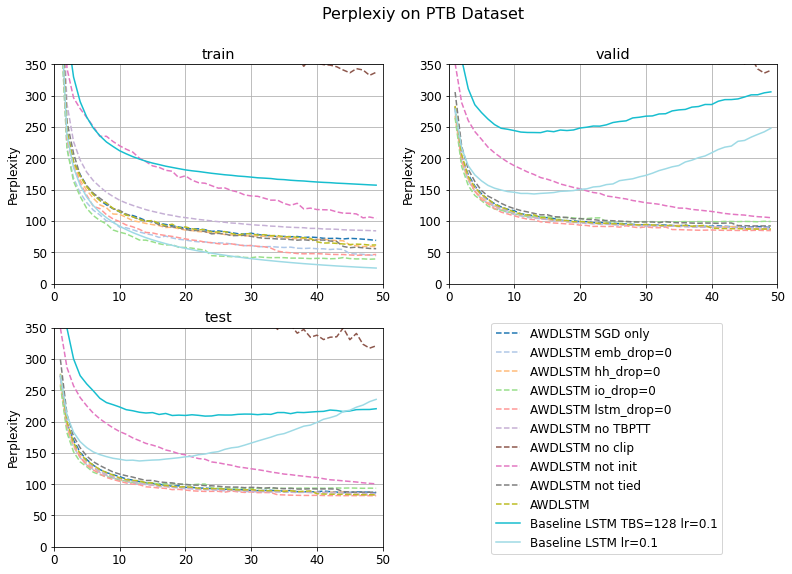
\includegraphics[scale=0.28]{assets/run_results.png}
    \vspace{-1.0em}
    \caption{Perplexity per epoch on PTB train, valid, and test sets}
    \vspace{-1.0em}
    \label{fig:results}
\end{figure}

\Cref{fig:results} shows the results of the several runs that have been performed, mostly to understand the effect of the regularisation and optimisation techniques that have been introduced.

By first analysing the \textit{Baseline}, it is possible to see how easily such model overfits, reaching astonishing performance on the training set by essentially memorising the data, but catastrophic results on the valid and test set.

Starting from such evidence, it was obvious that to improve the performance more regularisation techniques were needed. This led to the current AWD-LSTM implementation, which is explained more in detail in \Cref{sec:model}. The results obtained by considering such a model are obviously better; however, there are still some really interesting behaviours when analysing one by one the regularisation techniques.

To my surprise, I was actually very intrigued by how much performance changed whenever weight initialisation (i.e. \textit{AWDLSTM not init}) and clipping (i.e. \textit{AWDLSTM no clip}) were not performed. Of course, starting from a more favourable position leads to better results, explaining why weight initialisation is particularly important (i.e. the model converges faster and reaches a better local minimum). Instead, clipping the gradient is mandatory to avoid \textit{exploding gradient} when considering AWD-LSTM, given the fact that the shared parameters used during backpropagation start to become quite a few, causing such an undesired effect.

\begin{figure}
    \centering
    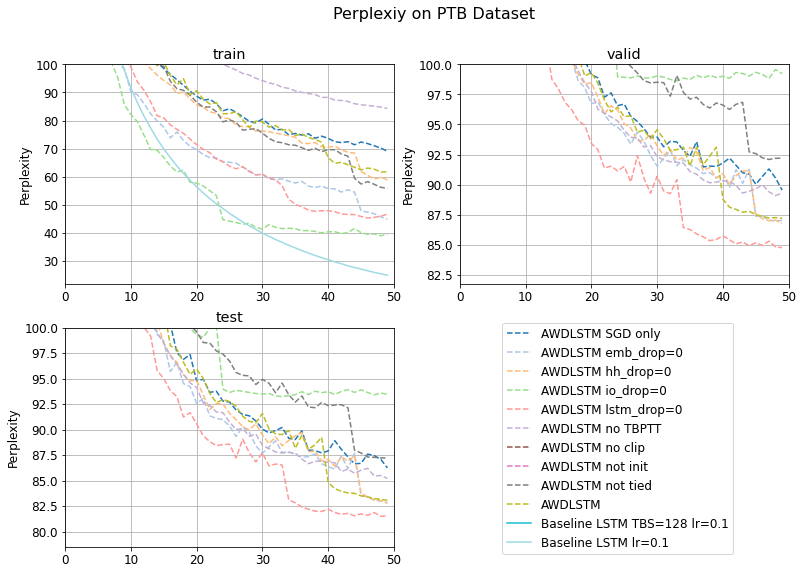
\includegraphics[scale=0.28]{assets/run_results_zoom_in.png}
    \vspace{-1.5em}
    \caption{Perplexity per epoch on PTB train, valid, and test sets (best runs details)}
    \vspace{-1.5em}
    \label{fig:results-zoom}
\end{figure}

\Cref{fig:results-zoom} shows a zoom-in of the previous image, depicting how the best techniques differ one from another in terms of performance. As it is possible to notice, they are all pretty close; however, we can see how
\begin{itemize}
\item without applying locked dropout (i.e. \textit{AWDLSTM io\_drop=0}) between both the embedding dropout and the classification layers, the model tends to overfit more on the training set, while obtaining worse performance on the validation and test set;
\item without parameters tying between the embedding and the classification layer (i.e. \textit{AWDLSTM not tied}) we achieve worse performance since the model is required to learn more parameters;
\item without ASGD (i.e. \textit{AWDLSTM SGD only}) convergence to the optimum is slower (i.e. the other runs benefit of the average).
\end{itemize}

\subsection{Error analysis}
To understand the reason why a model obtained certain performances, I tried to look at the length of the sentences that obtained better and worse results w.r.t. the average perplexity. The general idea was to find a correlation between a certain length and a possible source of error, e.g. discovering that the majority of short sentences were wrongly predicted. However, their distribution was pretty much identical in all the sets, meaning that sentences with different lengths appeared in both the splits.

\begin{figure}[!t]
    \centering
    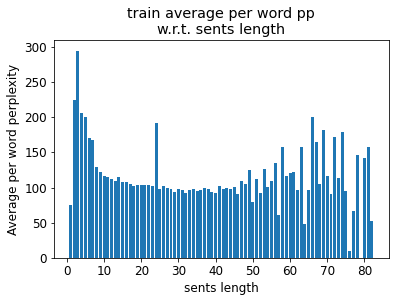
\includegraphics[scale=0.40]{assets/baseline_train_pp_per_length.png}
    \vspace{-1.0em}
    \caption{Baseline average perplexity per sentence length on the train set}
    \vspace{-1.0em}
    \label{fig:baseline-train-pp}
\end{figure}

\begin{figure}[!t]
    \centering
    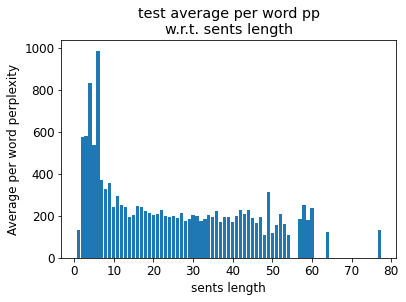
\includegraphics[scale=0.40]{assets/baseline_test_pp_per_length.png}
    \vspace{-1.0em}
    \caption{Baseline average perplexity per sentence length on the test set}
    \vspace{-1.0em}
    \label{fig:baseline-test-pp}
\end{figure}

\begin{figure}[!t]
    \centering
    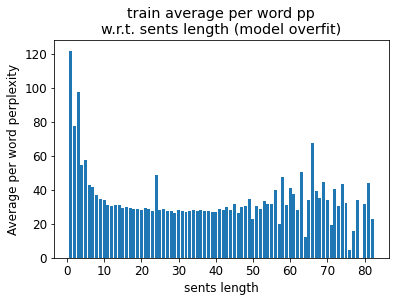
\includegraphics[scale=0.40]{assets/overfit_train_pp_per_length.png}
    \vspace{-1.0em}
    \caption{Baseline (overfit) average perplexity per sentence length on the train set}
    \vspace{-1.0em}
    \label{fig:overfit-train-pp}
\end{figure}

\begin{figure}[!t]
    \centering
    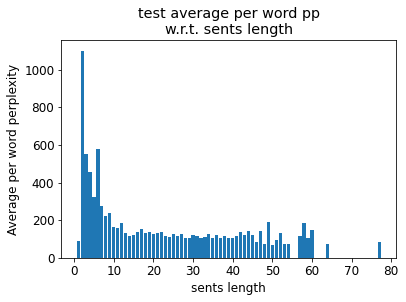
\includegraphics[scale=0.40]{assets/awdlstm_test_pp_per_length.png}
    \vspace{-1.0em}
    \caption{AWD-LSTM average perplexity per sentence length on the test set}
    \vspace{-1.0em}
    \label{fig:awdlstm-test-pp}
\end{figure}

Then, I looked at the average per word perplexity associated with sentences having a certain length. From this second analysis, a more interesting behaviour was discovered. \Cref{fig:baseline-train-pp} and \Cref{fig:baseline-test-pp} show its results on the baseline model on the train and test set respectively. From here we can observe two things: first of all, in both figures we can see that the model has a higher perplexity for shorter sentences; secondly, on the training set we also seem to have an issues with longer sentences.

Starting from the second issue, I decided to take a look at the results of the Baseline model that overfitted. In fact, I suspected that such behaviour was simply the result of a lack of training on the data, due to my early stopping criterion. In fact, by looking at \Cref{fig:overfit-train-pp} we can see that such behaviour has not completely disappeared, but has been greatly reduced. Moreover, another thing that can be considered is that the Baseline model has only a single recurrent layer and a limited embedding dimension, meaning that it can only capture context up to a certain length. Indeed, such behaviour is not present in AWD-LSTM.

Instead, shorter sentences seem to remain an issue even for AWD-LSTM, as shown in \Cref{fig:awdlstm-test-pp}. For this reason, I have decided to take a look at the word distribution that characterises sentences with at most 6 words. Thanks to such an analysis, I discovered why the model performed poorly: in fact, the most frequent words are the `\texttt{<unk>}' tag, the determinants, and the to be verb. This means that the possible continuations of sentences characterised by such words are extremely situational; meaning that the model can indeed find the best follow-up word for the training set by overfitting; but, it will have no chance of reaching good performance on the validation and test data if such follow-ups do not hold anymore.


\section{Conclusion}
\label{sec:conclusion}
To summarise, the Baseline LSTM obtained $137$ PP on the test set of the Word-level PTB dataset, but showed high overfitting. Such behaviour was corrected by embedding several regularisation techniques in the proposed implementation of AWD-LSTM. This, together with the usage of NT-ASGD, and TBPTT with variable length led to an accuracy of $81.43$ PP. Finally, possible follow-up works should focus on better handling shorter sentences, being them the main cause of errors.



\bibliographystyle{IEEEtran}

\bibliography{bibliography/mybib}

\end{document}
